% !TEX program = xelatex

\documentclass[12pt, a4paper, oneside]{ctexart}
\usepackage{amsmath, amsthm, amssymb, appendix, bm, graphicx, hyperref, mathrsfs}
\usepackage{float}
\usepackage{fontspec}
\usepackage{ctex}
\usepackage{enumitem}
\usepackage{subfigure,subcaption}
\usepackage{marvosym,tipa}
\usepackage{fancyhdr}
\usepackage[margin=1.25in]{geometry}
\setCJKmainfont{FandolSong}


% 设置页眉和页脚
\pagestyle{fancy}
\fancyhf{}
\fancyhead[L]{\rightmark} 
\fancyhead[C]{}
\fancyhead[R]{\thepage}
\renewcommand{\headrulewidth}{0.4pt}


\title{\textbf{Wugling 命题\\手语中的语言学}}
\author{陈王子\\https://www.zhihu.com/people/phlins\\princechen0116@gmail.com\\Copyright © 2024 Wangzi Chen. All rights reserved.}
\date{\today}
\linespread{1.5}

\begin{document}

\maketitle

\setcounter{page}{0}
\maketitle
\thispagestyle{empty}
\newpage
\tableofcontents
\listoffigures
\newpage

\section{选择题}

\subsection{语音题:香港手语的语音演变}
\begin{figure}[H]
    \centering
    \subfigure[i]{
    \begin{minipage}[t]{0.45\linewidth}
    \centering
    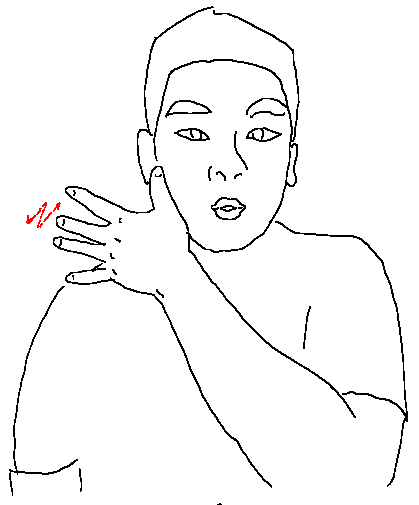
\includegraphics[width=\linewidth]{fig/fish2.pdf}
    %\caption{fig1}
    \end{minipage}%
    }%
    \subfigure[e]{
    \begin{minipage}[t]{0.45\linewidth}
    \centering
    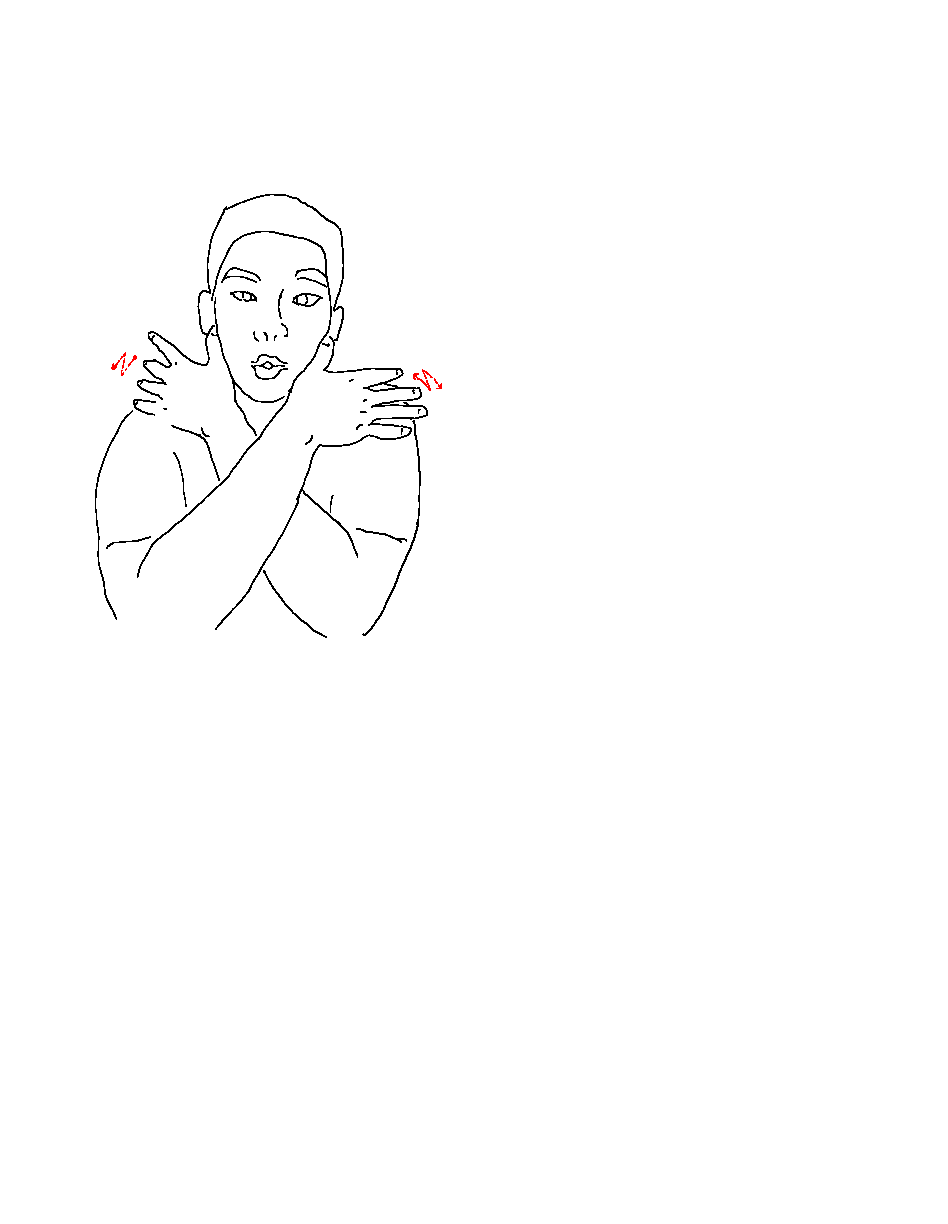
\includegraphics[width=\linewidth]{fig/fish1.pdf}
    %\caption{fig2}
    \end{minipage}%
    }%

                     
    \subfigure[\textrevepsilon]{
    \begin{minipage}[t]{0.45\linewidth}
    \centering
    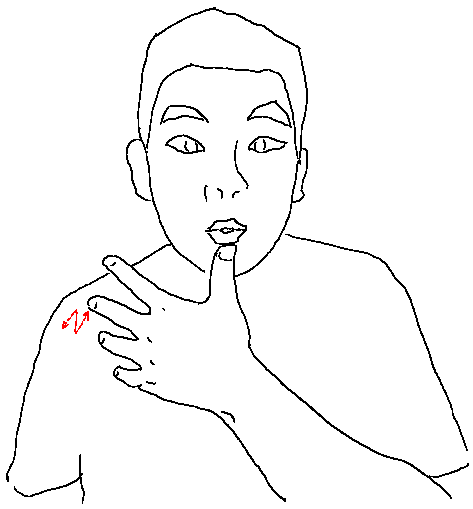
\includegraphics[width=\linewidth]{fig/fish4.pdf}
    %\caption{fig2}
    \end{minipage}
    }%
    \subfigure[a]{
    \begin{minipage}[t]{0.45\linewidth}
    \centering
    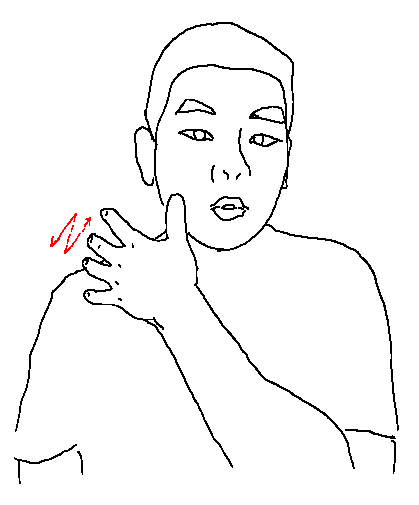
\includegraphics[width=\linewidth]{fig/fish3.pdf}
    %\caption{fig2}
    \end{minipage}
    }%
    \centering
    \caption{香港手语「鱼」}
    \label{fig:香港手语「鱼」}
\end{figure}

\paragraph{第一问}
【单选】图\ref{fig:香港手语「鱼」}是香港手语「鱼」的语音变化各阶段,该词汇呈现出简化调音的趋势。根据该描述,排序该词汇语音的发展历程。
\begin{enumerate}[label=\Alph*.]
    \item i-e-\textrevepsilon-a
    \item e-i-\textrevepsilon-a
    \item a-\textrevepsilon-e-i
    \item e-i-a-\textrevepsilon
\end{enumerate}
% 正确答案:D
\paragraph{第二问}
【多选】图\ref{fig:香港手语「鱼」}体现了手语中哪些语音演变规律?
\begin{enumerate}[label=\Alph*.]
    \item 删音(deletion):辅手脱落(weak drop),双手变为单手
    \item 动作向惯用手靠拢(dominant hand)
    \item 增音(epenthesis):辅手延展(weak hand spreading),单手变为双手
    \item 动作向非惯用手(辅手)靠拢(non-dominant hand, weak hand)
\end{enumerate}
% 正确答案:A,B
\paragraph{第三问}
【单选】上述单手手势中,左利手通常用他们的左手打,而右利手则用右手打,但意思没有任何不同。请问这构成了什么区别?
\begin{enumerate}[label=\Alph*.]
    \item 调音(articulation)
    \item 音位(phoneme)
    \item 语素(morpheme)
    \item 词根(root)
\end{enumerate}
% 正确答案:A
\newpage
\paragraph{第四问}
【单选】图\ref{fig:香港手语「11」}为香港手语词汇「11」,请问哪个香港手语词汇更古老?
\begin{enumerate}[label=\Alph*.]
    \item 手势\#2更老,手势\#1更新
    \item 该手势是同一手势的音位变体,完全没有新旧之分
    \item 手势\#1更老,手势\#2更新
    \item 以上说法都不对
\end{enumerate}
% 正确答案:C

\begin{figure}[H]
    \centering
    \subfigure[手势\#1开始状态]{
    \begin{minipage}[t]{0.5\linewidth}
    \centering
    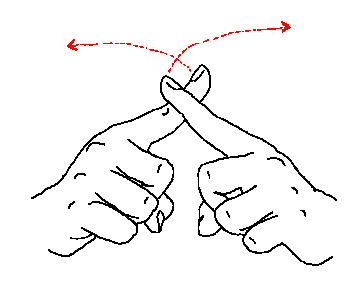
\includegraphics[width=\linewidth]{fig/11old1.pdf}
    %\caption{fig1}
    \end{minipage}%
    }%
    \subfigure[手势\#1结束状态]{
    \begin{minipage}[t]{0.5\linewidth}
    \centering
    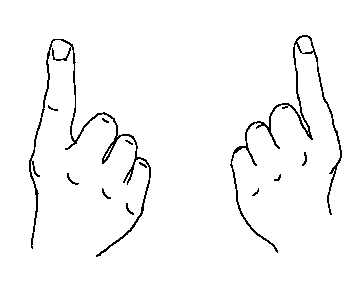
\includegraphics[width=\linewidth]{fig/11old2.pdf}
    %\caption{fig2}
    \end{minipage}%
    }%

    \centering
    \subfigure[手势\#2]{
        \begin{minipage}[t]{\linewidth}
        \centering
        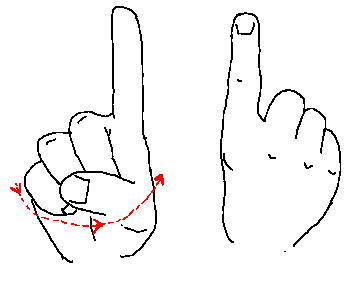
\includegraphics[width=0.5\linewidth]{fig/11new.pdf}
        %\caption{fig2}
        \end{minipage}%
    }%
    \caption{香港手语「11」}
    \label{fig:香港手语「11」}
\end{figure}



\subsection{音系题:中国手语中的音系学}
\begin{figure}[H]
    \centering
    \centering
    \subfigure[「方法」的第一个动作,意为方形]{
    \begin{minipage}[t]{0.5\linewidth}
    \centering
    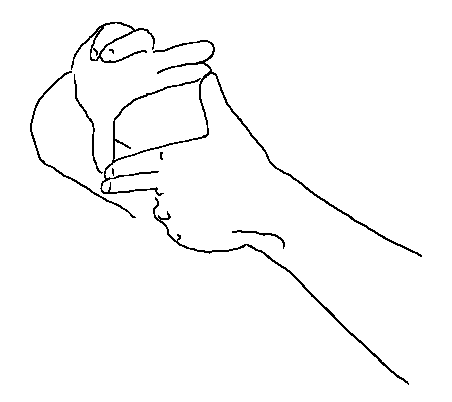
\includegraphics[width=\linewidth]{fig/fangfa1.pdf}
    %\caption{fig1}
    \end{minipage}%
    \label{fig:fangfa1}%
    }%
    \subfigure[「方法」的第二个动作,意为法律]{
    \begin{minipage}[t]{0.5\linewidth}
    \centering
    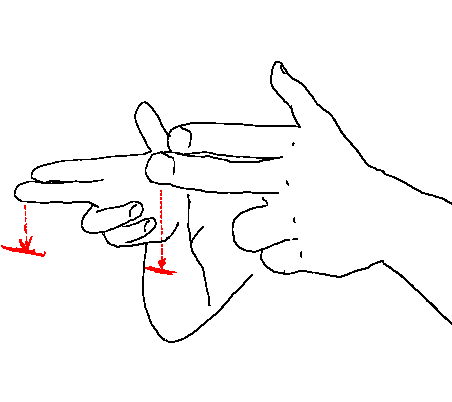
\includegraphics[width=\linewidth]{fig/fangfa2.pdf}
    %\caption{fig2}
    \end{minipage}%
    \label{fig:fangfa2}%
    }%
    \centering
    \caption{语流中的中国手语「方法」}
    \label{fig:语流中的中国手语「方法」}
\end{figure}

\begin{figure}[H]
    \centering
    \centering
    \subfigure[可能的F指拼\#1]{
    \begin{minipage}[t]{0.4\linewidth}
    \centering
    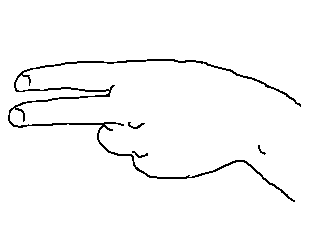
\includegraphics[width=\linewidth]{fig/f.pdf}
    %\caption{fig1}
    \end{minipage}%
    \label{fig:F指拼}%
    }%
    \subfigure[可能的F指拼\#2]{
    \begin{minipage}[t]{0.4\linewidth}
    \centering
    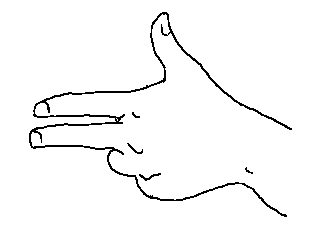
\includegraphics[width=\linewidth]{fig/f+1.pdf}
    %\caption{fig2}
    \end{minipage}%
    \label{fig:F指拼+1}%
    }%

    \centering
    \subfigure[可能的「方形」]{
        \begin{minipage}[t]{\linewidth}
        \centering
        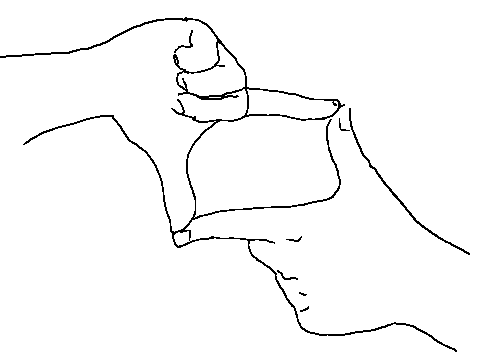
\includegraphics[width=0.4\linewidth]{fig/fang.pdf}
        %\caption{fig2}
        \end{minipage}%
        \label{fig:方形}%
    }%
    \centering
    \caption{手指拼音和词汇}
    \label{fig:手指拼音和词汇}
\end{figure}

\paragraph{第一问}
【单选】图\ref{fig:语流中的中国手语「方法」}是一位聋人在语流中打出的的「方法」(fāngfǎ,way,method)。请问图\ref{fig:手指拼音和词汇}中,哪项为「方形」,
哪项为手指拼音「F」?在以上两个语素中,聋人都伸出了一根多余的手指,这种音系学现象叫什么名字?

\begin{enumerate}[label=\Alph*.]
    \item 图\ref{fig:方形}为方形,图\ref{fig:F指拼+1}为F指拼,现象叫逆同化(regressive assimilation)
    \item 图\ref{fig:fangfa1}为方形,图\ref{fig:F指拼+1}为F指拼,现象叫异化(dissimilation)
    \item 图\ref{fig:方形}为方形,图\ref{fig:F指拼}为F指拼,现象叫同化(assimilation)
    \item 图\ref{fig:fangfa1}为方形,图\ref{fig:F指拼}为F指拼,现象叫异化(dissimilation)
\end{enumerate}
% regressive handshape assimilation
% 答案为:C




\begin{figure}[H]
    \centering
    \centering
    \subfigure[手型\#0]{
    \begin{minipage}[t]{0.33\linewidth}
    \centering
    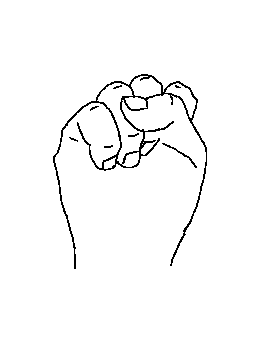
\includegraphics[width=\linewidth]{fig/unmarked0.pdf}
    %\caption{fig1}
    \end{minipage}%
    \label{fig:unmarked0}%
    }%
    \subfigure[手型\#1]{
    \begin{minipage}[t]{0.33\linewidth}
    \centering
    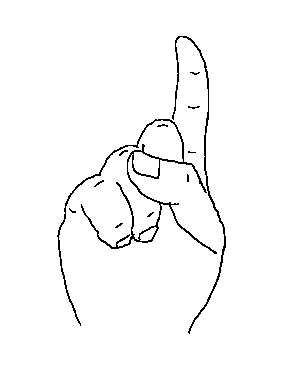
\includegraphics[width=\linewidth]{fig/unmarked1.pdf}
    %\caption{fig2}
    \end{minipage}%
    \label{fig:unmarked1}%
    }%
    \subfigure[手型\#2]{
        \begin{minipage}[t]{0.33\linewidth}
        \centering
        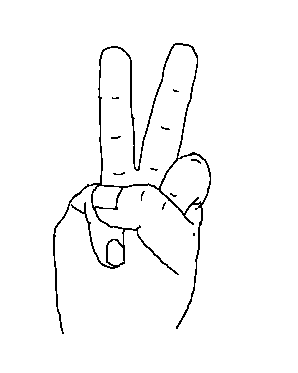
\includegraphics[width=\linewidth]{fig/marked2.pdf}
        %\caption{fig2}
        \end{minipage}%
        \label{fig:marked2}%
    }%

    \subfigure[手型\#3]{
        \begin{minipage}[t]{0.33\linewidth}
        \centering
        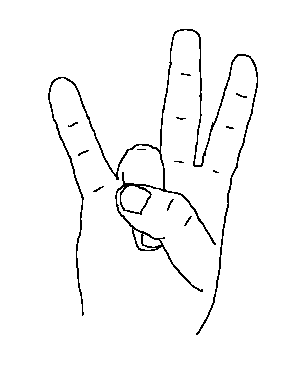
\includegraphics[width=\linewidth]{fig/marked3.pdf}
        %\caption{fig1}
        \end{minipage}%
        \label{fig:marked3}%
        }%
        \subfigure[手型\#5]{
        \begin{minipage}[t]{0.33\linewidth}
        \centering
        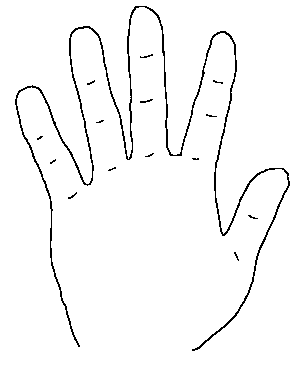
\includegraphics[width=\linewidth]{fig/unmarked5.pdf}
        %\caption{fig2}
        \end{minipage}%
        \label{fig:unmarked5}%
        }%
        \centering
    \caption{不同手型}
    \label{fig:不同手型}
\end{figure}

\paragraph{第二问}
【单选】儿童第一批习得的手型往往是简单、自然的无标记手型(unmarked handshape)。下面哪几个手型有标记?
\begin{enumerate}[label=\Alph*.]
    \item 图\ref{fig:unmarked0}手型\#0、图\ref{fig:unmarked1}手型\#1、图图\ref{fig:unmarked5}手型\#5
    \item 图\ref{fig:marked2}手型\#2、图\ref{fig:marked3}手型\#3
    \item 图\ref{fig:unmarked1}手型\#1、图\ref{fig:marked2}手型\#2、图\ref{fig:marked3}手型\#3
    \item 图\ref{fig:unmarked0}手型\#0、图\ref{fig:unmarked5}手型\#5
\end{enumerate}
% 答案:B

\paragraph{第三问}
\begin{figure}[H]
    \centering
    \centering
    \subfigure[南非手语词汇\#1]{
    \begin{minipage}[t]{0.5\linewidth}
    \centering
    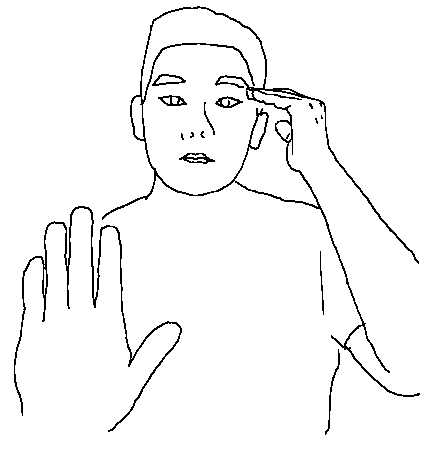
\includegraphics[width=\linewidth]{fig/know.pdf}
    %\caption{fig1}
    \end{minipage}%
    \label{fig:know}%
    }%
    \subfigure[南非手语词汇\#2]{
    \begin{minipage}[t]{0.5\linewidth}
    \centering
    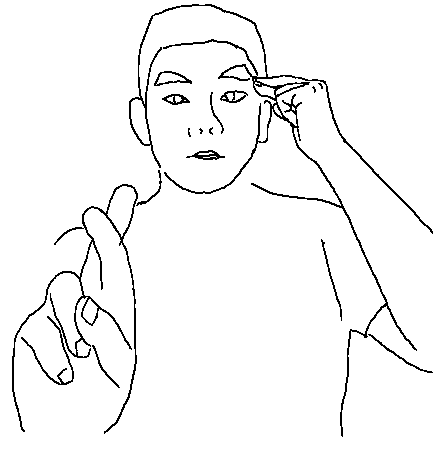
\includegraphics[width=\linewidth]{fig/remember.pdf}
    %\caption{fig2}
    \end{minipage}%
    \label{fig:remember}%
    }%
    \centering
    \caption{南非手语中的「知道」和「记得」}
    \label{fig:南非手语}
\end{figure}

【单选】图\ref{fig:南非手语}为南非手语中的「知道」和「记得」,左下展示了右手的手型,「记得」的手型有标记。哪一个手势是「知道」?聋人在快速语流中,可能会将这两个手势均简化为哪个手势?
\begin{enumerate}[label=\Alph*.]
    \item 图\ref{fig:remember}为「知道」,均简化为图\ref{fig:remember}
    \item 图\ref{fig:know}为「知道」,均简化为图\ref{fig:know}
    \item 图\ref{fig:remember}为「知道」,均简化为图\ref{fig:know}
    \item 图\ref{fig:know}为「知道」,均简化为图\ref{fig:remember}
\end{enumerate}
% 答案:B

\subsection{语言接触:中国手语的语言接触}
\paragraph{第一问}
\begin{figure}[H]
    \centering
    \subfigure[墨]{
    \begin{minipage}[t]{0.33\linewidth}
    \centering
    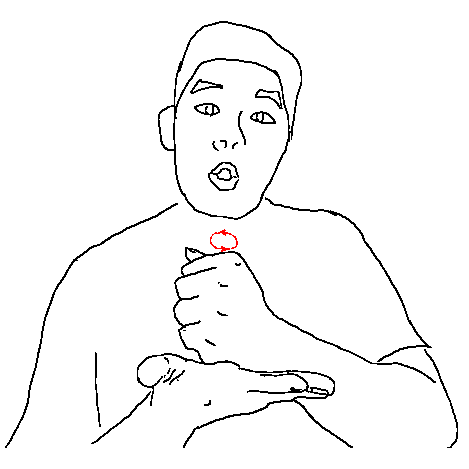
\includegraphics[width=\linewidth]{fig/moxige1.pdf}
    %\caption{fig1}
    \end{minipage}%
    \label{fig:mo}%
    }%
    \subfigure[四]{
    \begin{minipage}[t]{0.33\linewidth}
    \centering
    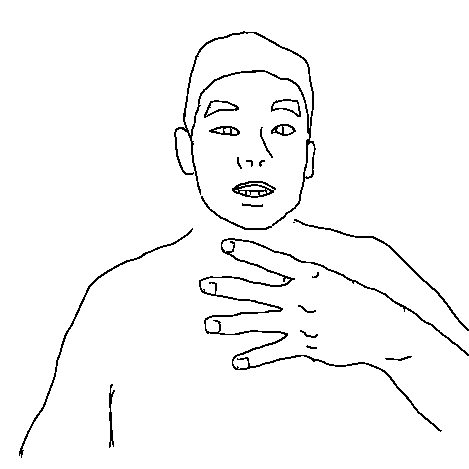
\includegraphics[width=\linewidth]{fig/moxige2.pdf}
    %\caption{fig2}
    \end{minipage}%
    \label{fig:si}%
    }%
    \subfigure[哥哥]{
        \begin{minipage}[t]{0.33\linewidth}
        \centering
        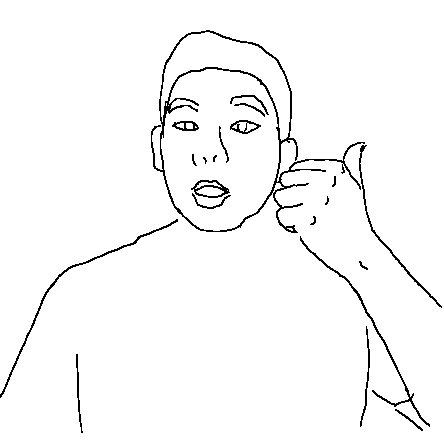
\includegraphics[width=\linewidth]{fig/moxige3.pdf}
        %\caption{fig2}
        \end{minipage}%
        \label{fig:gege}%
    }%
    \caption{北京手语「墨西哥」}
    \label{fig:北京手语「墨西哥」}
\end{figure}
【单选】语言接触时会发生借用(borrowing):借词(loanword)属于直接借用了源语言的形式(如「咖啡」),而仿译(loan translations/calque)则属于将源语言直译组装(如「热狗」)。图\ref{fig:北京手语「墨西哥」}为北京聋人所打的「墨西哥」。用「四」指代「西」属于什么语言接触现象?整个词汇反映了什么语言接触现象?
\begin{enumerate}[label=\Alph*.]
    \item 仿译、仿译
    \item 仿译、借词
    \item 借词、借词
    \item 借词、仿译
\end{enumerate}
% 答案:A

\paragraph{第二问}
【单选】在中国手语(国家通用手语)中,「消防」的一种打法为「火/扑灭」,但「消防车」的打法为「扑灭/火/带警示灯的车辆」。近一百年来,美国手语的语序由主宾谓逐渐变为主谓宾。这两个例子说明了什么现象?
\begin{enumerate}[label=\Alph*.]
    \item 双言现象(diglossia situation)
    \item 语码融合(code-mixing)
    \item 语言接触导致的特征转移(feature transfer)
    \item 连续体(continuum)
\end{enumerate}
% 答案:C

\newpage
\subsection{心理语言学:手语中的时间}

% 隐喻:现在和未来(214)

\begin{figure}[H]
    \centering
    \centering
    \subfigure[中国手语词汇\#1]{
    \begin{minipage}[t]{0.5\linewidth}
    \centering
    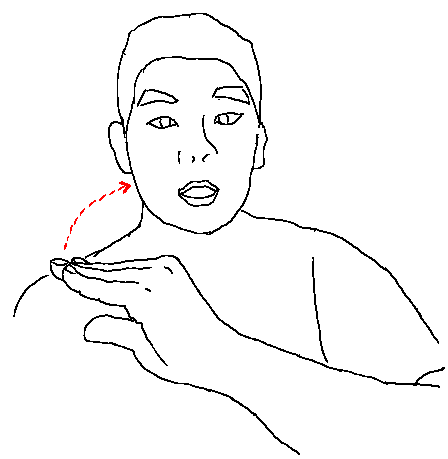
\includegraphics[width=\linewidth]{fig/zao.pdf}
    %\caption{fig1}
    \end{minipage}%
    \label{fig:zao}%
    }%
    \subfigure[中国手语词汇\#2]{
    \begin{minipage}[t]{0.5\linewidth}
    \centering
    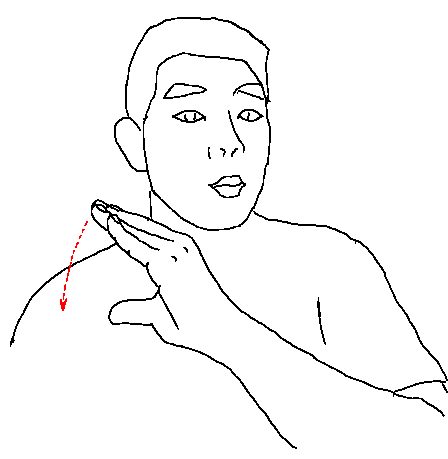
\includegraphics[width=\linewidth]{fig/wan.pdf}
    %\caption{fig2}
    \end{minipage}%
    \label{fig:wan}%
    }%
    \centering
    \caption{中国手语中的「早晨」和「晚上」}
    \label{fig:中国手语中的「早晨」和「晚上」}
\end{figure}

\paragraph{第一问}
【单选】图\ref{fig:中国手语中的「早晨」和「晚上」}表示中国手语(国家通用手语)中的「早晨」和「晚上」。哪个是「早晨」?哪个是「晚上」?他们象征着哪颗天体的运动?

\begin{enumerate}[label=\Alph*.]
    \item 图\ref{fig:zao}是「早晨」,图\ref{fig:wan}是「晚上」,象征着月亮
    \item 图\ref{fig:wan}是「早晨」,图\ref{fig:zao}是「晚上」,象征着月亮
    \item 图\ref{fig:zao}是「早晨」,图\ref{fig:wan}是「晚上」,象征着太阳
    \item 图\ref{fig:wan}是「早晨」,图\ref{fig:zao}是「晚上」,象征着太阳
\end{enumerate}
% 答案:C

\newpage

\paragraph{第二问}
【单选】图\ref{fig:中国手语中的「昨天」}所示为中国手语(国家通用手语)中的「昨天」。将相对空间位置上的「前后」借用为相对时间位置上的「前后」,这种语言现象叫什么名字?
\begin{enumerate}[label=\Alph*.]
    \item 转喻(metonymy)
    \item 拟人(personification)
    \item 借代(synecdoche)
    \item 隐喻(metaphor)
\end{enumerate}
% 答案:D

\begin{figure}[H]
    \centering
    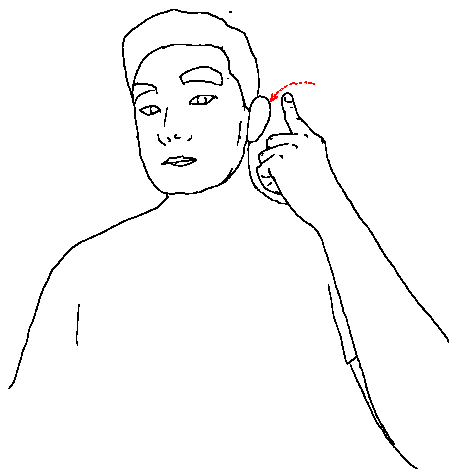
\includegraphics[width=0.66\linewidth]{fig/zuotian.pdf}
    \centering
    \caption{中国手语中的「昨天」}
    \label{fig:中国手语中的「昨天」}
\end{figure}

\paragraph{第三问}
【多选】根据上面两问,请问中国手语中的时间线流向至少有哪几种?
\begin{enumerate}[label=\Alph*.]
    \item \textbf{从背后向身前}
    \item \textbf{从身前向背后}
    \item \textbf{从低到高的生长线}
    \item \textbf{位于身前的天体运行线}
\end{enumerate}
% 答案:A,D


% 各语言对时间流动的方向看法不同。手语中大概有四种时间线流向:
% \begin{enumerate}
%     \item \textbf{从背后向身前}:如美国手语中 PAST 位于身后,而 FUTURE 在身前。
%     \item \textbf{从身前向背后}:如 Urubu-Kaapor 手语认为「过去」是「已经看见的」,所以位于身前;「未来」理解为「看不到的」,所以位于身后。可类比汉语「以前」「以后」。
%     \item \textbf{从低到高的生长线}:如Adamorobe 手语。
%     \item \textbf{位于身前的天体运行线}:中国手语中的早晨、晚上。
% \end{enumerate}

\newpage
\subsection{句法学:省略与代指}
\begin{figure}[H]
    \centering
    \subfigure[手语屈折\#1]{
    \begin{minipage}[t]{0.33\linewidth}
    \centering
    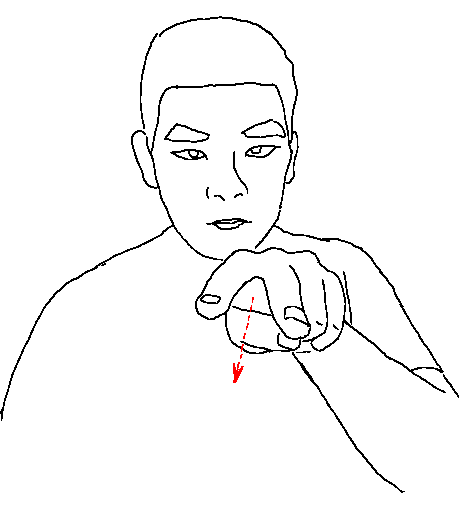
\includegraphics[width=\linewidth]{fig/ilook.pdf}
    %\caption{fig1}
    \end{minipage}%
    \label{fig:ilook}%
    }%
    \subfigure[手语屈折\#2]{
    \begin{minipage}[t]{0.33\linewidth}
    \centering
    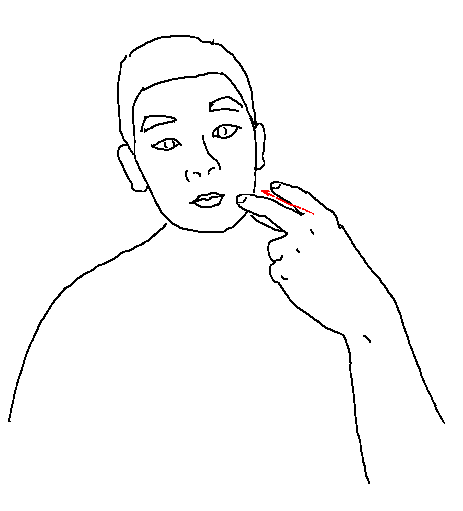
\includegraphics[width=\linewidth]{fig/youlook.pdf}
    %\caption{fig2}
    \end{minipage}%
    \label{fig:youlook}%
    }%
    \subfigure[手语屈折\#3]{
        \begin{minipage}[t]{0.33\linewidth}
        \centering
        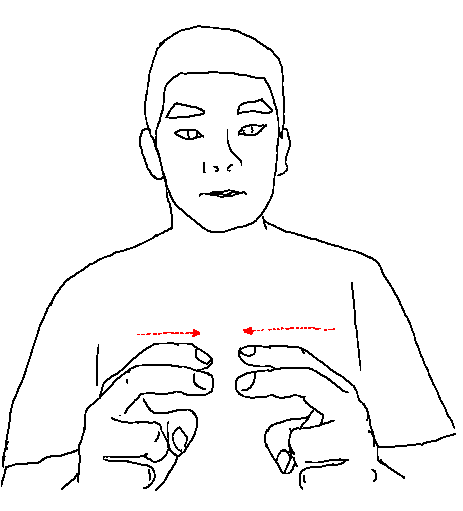
\includegraphics[width=\linewidth]{fig/2look.pdf}
        %\caption{fig2}
        \end{minipage}%
        \label{fig:2look}%
    }%
    \caption{中国手语中「看」的屈折}
    \label{fig:中国手语中「看」的屈折}
\end{figure}

\paragraph{第一问}
【单选】在图\ref{fig:中国手语中「看」的屈折}中,请问哪个手势是「我看你」?哪个是「你看我」?哪个是「两个人对看」?
\begin{enumerate}[label=\Alph*.]
    \item 图\ref{fig:youlook}是「我看你」,图\ref{fig:ilook}是「你看我」,图\ref{fig:2look}是「两个人对看」
    \item 图\ref{fig:youlook}是「我看你」,图\ref{fig:2look}是「你看我」,图\ref{fig:ilook}是「两个人对看」
    \item 图\ref{fig:ilook}是「我看你」,图\ref{fig:2look}是「你看我」,图\ref{fig:youlook}是「两个人对看」
    \item 图\ref{fig:ilook}是「我看你」,图\ref{fig:youlook}是「你看我」,图\ref{fig:2look}是「两个人对看」
\end{enumerate}
% 答案:D

\paragraph{第二问}
【单选】为什么中国手语允许代词脱落(pro-drop)?选择最恰当的解释。
\begin{enumerate}[label=\Alph*.]
    \item 聋人不重视代词的习惯导致代词随意脱落
    \item 一些手语动词的屈折形态蕴含了代词信息
    \item 手语的语法规则不够完善,所以允许代词脱落
    \item 手语动词都蕴含了论元,因此允许省略
\end{enumerate}
% 答案:B

\end{document}

